% ===============================================================
\section{Methodology}\label{sec:methodology}
% ===============================================================

\subsection{Problem Definition}\label{subsec:problem_definition}

Let $\mathcal{C}=\{D_1,\ldots,D_N\}$ denote the Vietnamese legal corpus of
$N$ documents. From $\mathcal{C}$, the system builds two complementary
knowledge sources: a dense vector index
$\mathcal{I}_v=\{(c_j,\mathbf{e}_j)\}_{j=1}^{M}$ of $M$ legal text chunks,
where $c_j$ is the $j$-th chunk and $\mathbf{e}_j\in\mathbb{R}^d$ is its
$d$-dimensional embedding; and a legal knowledge graph
$\mathcal{G}=(\mathcal{V},\mathcal{E})$ where a node $v\in\mathcal{V}$
represents a legal document, article, semantic concept, agency, or other
entity, and an edge $(u,r,v)\in\mathcal{E}$ represents a typed relation $r$
from source node $u$ to target node $v$, such as \textsc{HAS\_ARTICLE},
\textsc{MENTIONS}, \textsc{AMENDS}, or \textsc{REPLACES}. Table~\ref{tab:notation}
summarises the notation used throughout.

\begin{table}[!htbp]
\centering
\caption{Summary of notation}\label{tab:notation}
\begin{tabularx}{\columnwidth}{L{2.1cm}Y}
\toprule
\textbf{Symbol} & \textbf{Meaning} \\
\midrule
$\mathcal{C},\,\mathcal{I}_v,\,\mathcal{G}$ & legal corpus, dense index, knowledge graph \\
$q_t,\,H$ & query at turn $t$ and conversation history $H=\{(q_i,a_i)\}_{i=1}^{t-1}$ \\
$\mathcal{D}=\{d_v,d_g,d_h,d_c\}$ & route set: dense, graph, hybrid, clarify \\
$\rho$ & routing function $\rho(q_t,H)\!\to\! d^*\!\in\!\mathcal{D}$ \\
$E_{d^*},E_v,E_g$ & evidence set for route $d^*$; dense and graph evidence \\
$k,\,h$ & dense retrieval depth; maximum traversal depth \\
$\mathbf{f}(q_t,H,r_H)$ & feature vector, $\mathbf{f}\in\mathbb{R}^{n_f}$ \\
$\phi_{\mathrm{amb}}(q_t,H,r_H)$ & ambiguity score, $\in[0,1]$ \\
$\xi(q_t)$ & multi-hop score, $\in\{0,1,2\}$ \\
$r_H$ & history-resolution status (Eq.~\ref{eq:history_states}) \\
$f_1$ & Stage-1 classifier, outputs $(d_1,s_1)$ \\
$s_1$ & Stage-1 confidence (max softmax probability) \\
$\gamma_{\mathrm{conf}},\gamma_{\mathrm{amb}},\gamma_{\mathrm{hop}}$ & binary Stage-2 trigger indicators \\
$\Gamma$ & composite Stage-2 trigger \\
$\tau_{\mathrm{conf}},\tau_{\mathrm{force}},\tau_{\mathrm{clar}}$ & confidence, forcing, and clarify-override thresholds \\
$f_2$ & Stage-2 LLM verifier \\
$a_t,\,c_t$ & generated answer; clarification question \\
\bottomrule
\end{tabularx}
\end{table}

At inference time, the input is the current query $q_t$ at turn $t\geq 1$,
together with optional conversation history $H=\{(q_i,a_i)\}_{i=1}^{t-1}$
(empty when $t=1$). The router selects one action from the route set
\begin{equation}
\mathcal{D}=\{d_v,\,d_g,\,d_h,\,d_c\},
\label{eq:route_set}
\end{equation}
where $d_v$, $d_g$, $d_h$, $d_c$ denote \texttt{dense\_retrieval},
\texttt{graph\_traversal}, \texttt{hybrid\_reasoning}, and \texttt{clarify},
respectively. The router is modelled as a function $\rho$ mapping the input
pair to a route:
\begin{equation}
d^* = \rho(q_t,H),\qquad d^*\in\mathcal{D}.
\label{eq:routing_function}
\end{equation}
For the three retrieval routes, the evidence set $E_{d^*}$ is determined by
the selected route $d^*$:
\begin{equation}
E_{d^*}=
\begin{cases}
\mathrm{TopK}(q_t,\mathcal{I}_v,k) & \text{if } d^*=d_v,\\[3pt]
\mathrm{Traverse}(q_t,\mathcal{G},h) & \text{if } d^*=d_g,\\[3pt]
E_v\cup E_g & \text{if } d^*=d_h,
\end{cases}
\label{eq:evidence_set}
\end{equation}
where $E_v\triangleq\mathrm{TopK}(q_t,\mathcal{I}_v,k)$ is the set of the $k$
chunks most similar to $q_t$ in $\mathcal{I}_v$;
$E_g\triangleq\mathrm{Traverse}(q_t,\mathcal{G},h)$ is the evidence obtained
by linking entities in $q_t$ to nodes of $\mathcal{G}$ and traversing up to a
maximum depth $h$; $k\in\mathbb{N}^{*}$ is the dense retrieval depth (number
of top-$k$ chunks returned) and $h\in\mathbb{N}^{*}$ is the maximum traversal
depth. The clarify route $d_c$ produces no evidence set and therefore does
not appear in~\eqref{eq:evidence_set}. The generator then produces
$a_t=\mathrm{Generate}(q_t,H,E_{d^*})$. If $d^*=d_c$, no evidence is
retrieved; instead the system returns a clarification question
$c_t=\mathrm{Clarify}(q_t,H)$.

\subsection{Dataset}\label{subsec:dataset}

The evaluation uses a self-constructed Vietnamese legal QA routing dataset
derived from a single source: the Vietnamese electronic legal codification
system (\textit{Bộ Pháp điển điện tử}), flattened into article-level records.
Question--answer pairs were generated from sampled legal articles using the
Gemini API. For each text snippet, the model was prompted with templates
specific to the three evidence structures to synthesize realistic user
queries, and the exact corresponding span in the article was extracted as the
ground-truth answer. A subset of the generated pairs was then manually
reviewed to ensure legal soundness and prevent hallucinated facts.
QA pairs are linked to supporting articles through an \texttt{article\_key}
(format \texttt{DOC::ARTICLE\_ID}) and assigned routing labels based on
evidence structure: \texttt{dense\_retrieval} for single-article questions,
\texttt{graph\_traversal} for multi-article reasoning within one document,
and \texttt{hybrid\_reasoning} for evidence spanning multiple documents.
Low-quality samples are removed by deduplication, length filtering, and
placeholder-answer filtering. To reduce template-induced lexical leakage in
the routing features, the surface forms of the generated queries are
additionally paraphrased while preserving their underlying evidence
structure, so that the routing classifier must rely on genuine structural
signals rather than memorised template wording.

Table~\ref{tab:dataset} summarises the dataset splits. The dataset remains
skewed toward dense retrieval, which accounts for half of the samples
($50\%$; Fig.~\ref{fig:dataset_bar} shows the test-split distribution),
motivating Macro-F1 reporting alongside accuracy. The strict split
is used for retrieval-route evaluation; the \texttt{clarify} route is
evaluated separately on a $234$-query ambiguity benchmark ($156$ ambiguous,
$78$ answerable controls) and a $160$-query conversation stress test.
The $234$-query ambiguity dataset was constructed by systematically dropping
essential context (such as subjects or conditions) from well-posed queries to
form $156$ ambiguous samples, which were paired with $78$ unambiguous
controls authored by legal experts. The $160$-query conversation set was
synthesized to simulate realistic multi-turn dialogues encompassing topic
shifts and contextual references, followed by a human validation pass to
guarantee contextual coherence.

\begin{table}[!htbp]
\centering
\caption{Vietnamese legal QA routing dataset split}\label{tab:dataset}
\begin{tabular}{lrrrr}
\toprule
\textbf{Split} & \textbf{Dense} & \textbf{Graph} & \textbf{Hybrid} & \textbf{Total} \\
\midrule
Train & 400 & 200 & 200 & 800 \\
Dev   & 50  & 25  & 25  & 100 \\
Test  & 300 & 150 & 150 & 600 \\
\midrule
\textbf{Total} & 750 & 375 & 375 & 1{,}500 \\
\bottomrule
\end{tabular}
\end{table}

\begin{figure}[!htbp]
\centering
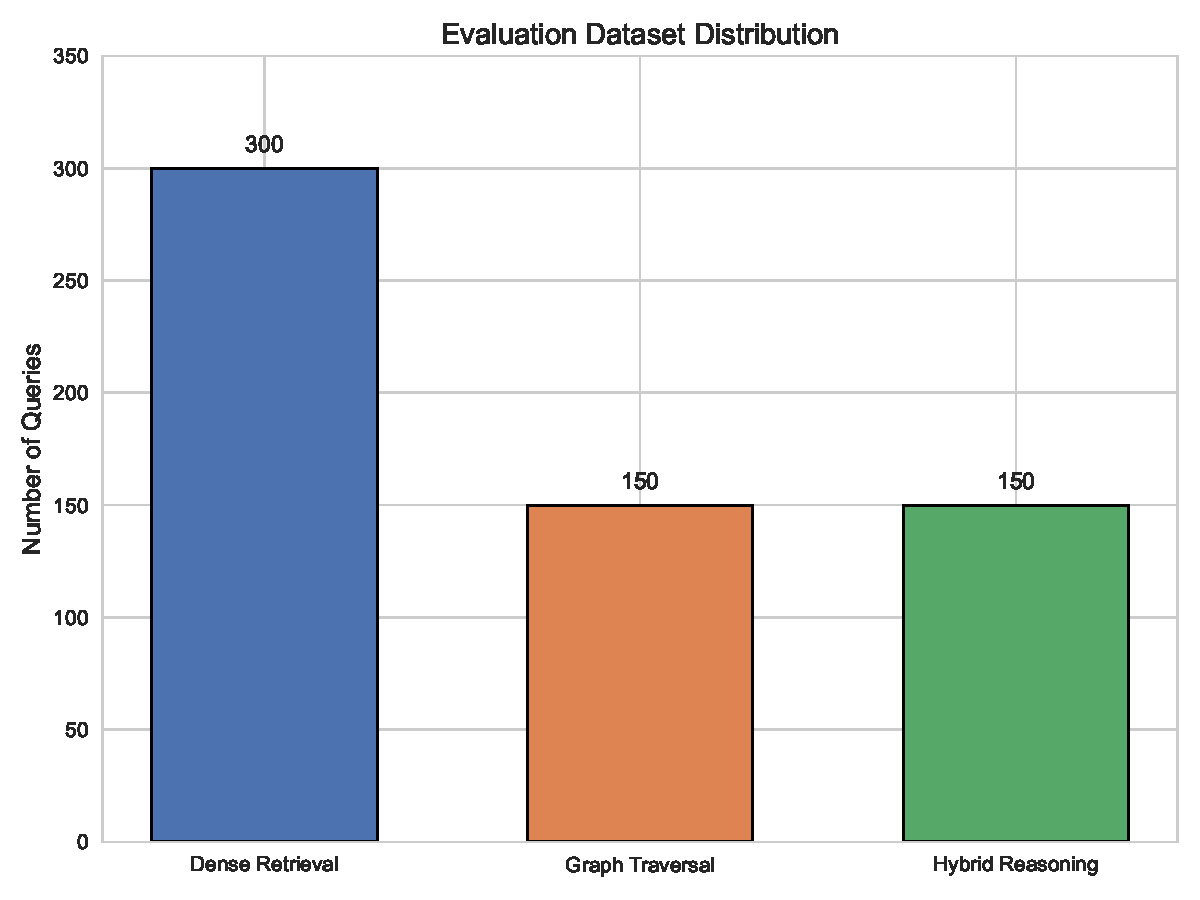
\includegraphics[width=0.85\columnwidth]{figs/dataset_bar.pdf}
\caption{Route-label distribution of the strict $600$-query evaluation set:
$300$ dense-retrieval, $150$ graph-traversal, and $150$ hybrid-reasoning
queries}\label{fig:dataset_bar}
\end{figure}

\subsection{System Overview}\label{subsec:system_overview}

% NOTE(M13): figs/*.jpg are raster. Springer prefers vector line art (EPS/PDF)
% or >=600 DPI for combination art. Re-export the draw.io diagrams as PDF/EPS
% and the bar chart as PDF; rename to Fig1..Fig4 on final submission.
\begin{figure}[!htbp]
\centering
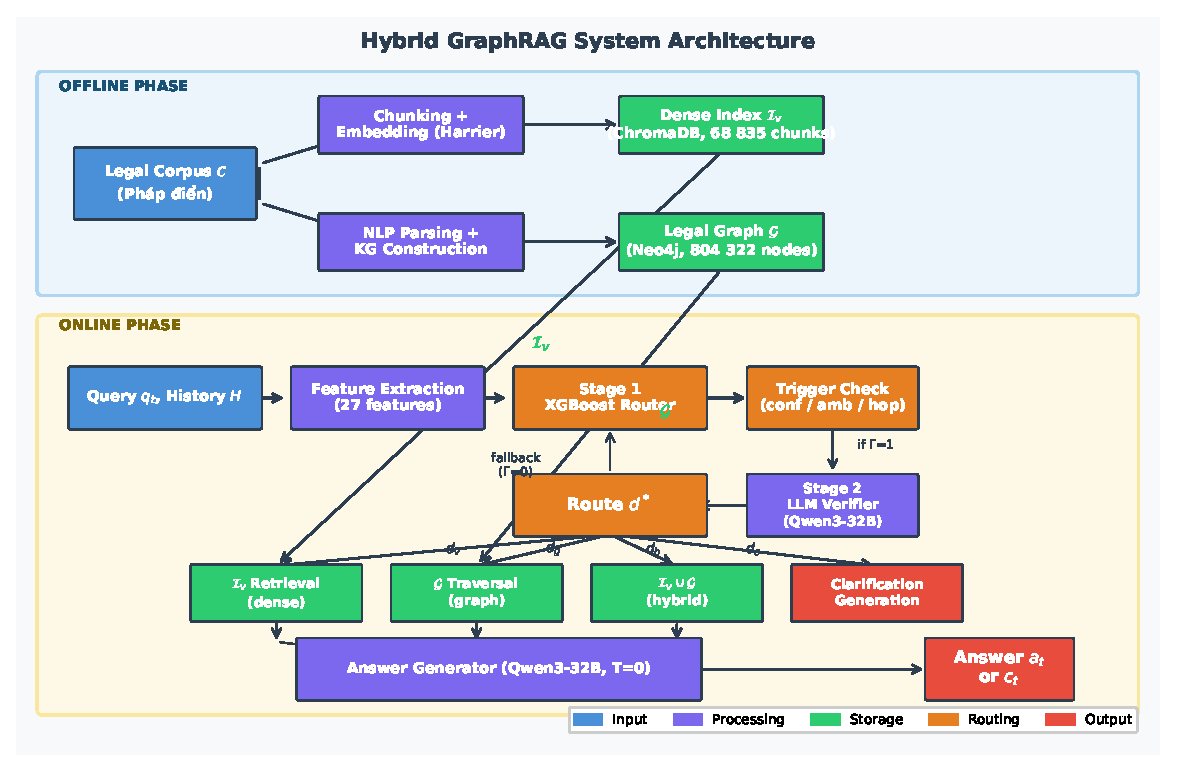
\includegraphics[width=\columnwidth]{figs/system_architecture}
\caption{High-level data flow of the proposed Hybrid GraphRAG system. The
Vietnamese legal corpus $\mathcal{C}$ is processed offline into a dense
vector index $\mathcal{I}_v$ (ChromaDB) and a legal knowledge graph
$\mathcal{G}$ (Neo4j). At query time the two-stage adaptive router selects
evidence from $\mathcal{I}_v$, $\mathcal{G}$, or both, or returns a
clarification question $c_t$. Box colours denote input, processing, storage,
routing, and output stages}\label{fig:system_architecture}
\end{figure}

\begin{figure*}[!htbp]
\centering
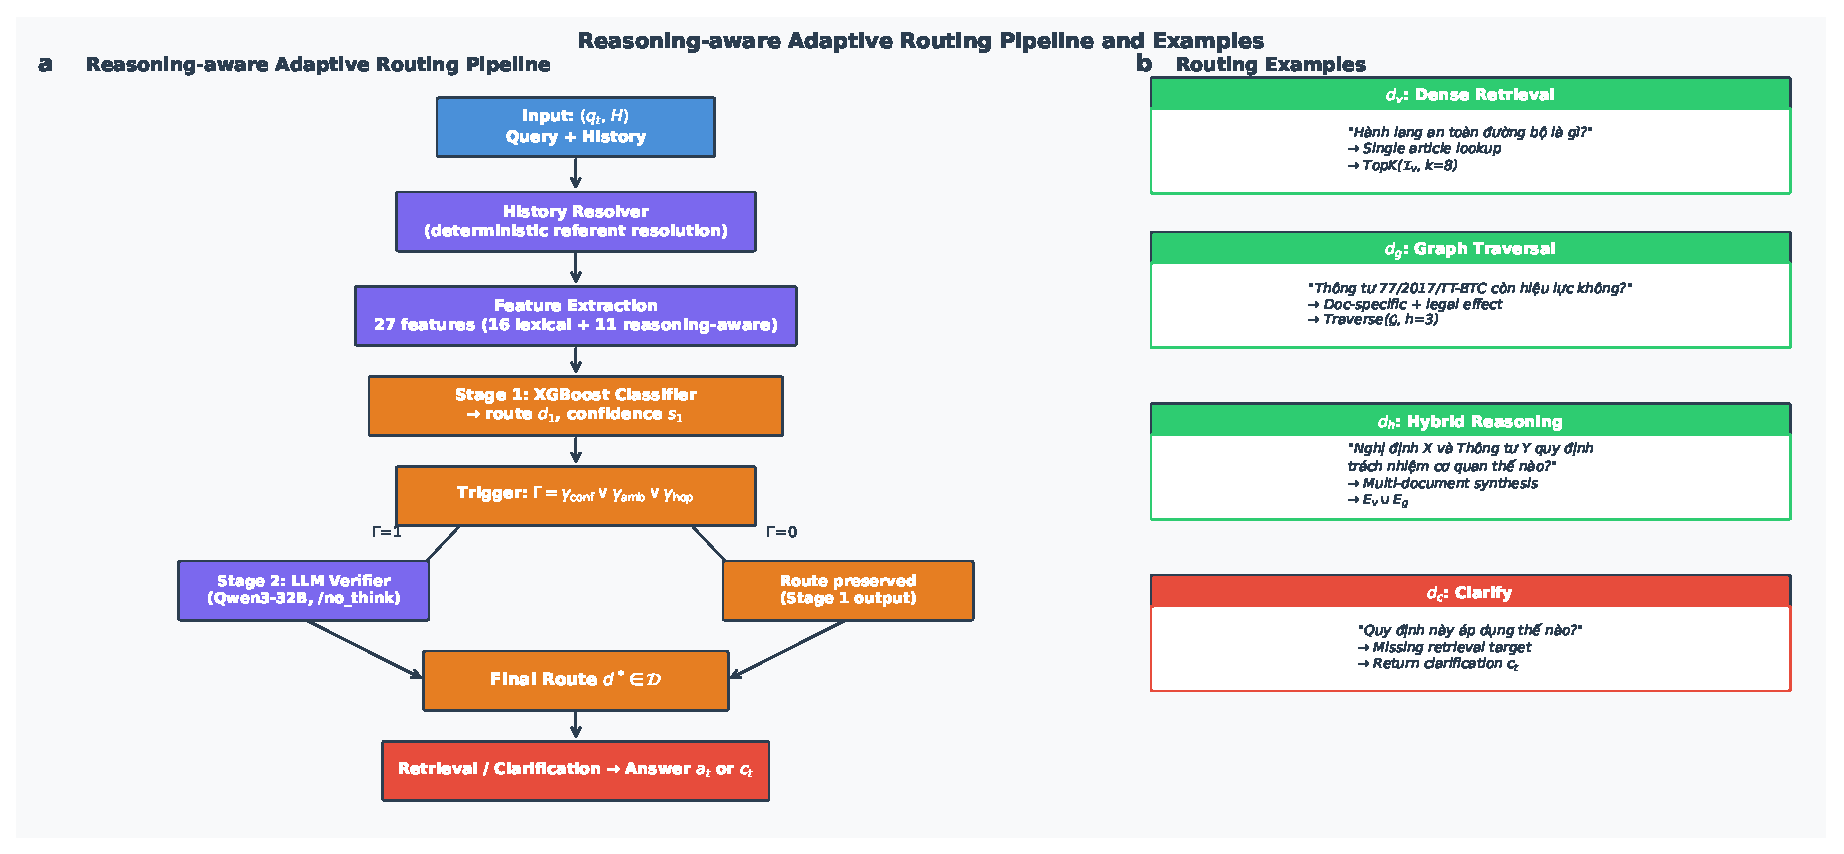
\includegraphics[width=\textwidth]{figs/system_pipeline}
\caption{Reasoning-aware adaptive routing pipeline and illustrative routing
outcomes. \textbf{a} The pipeline processes $(q_t,H)$ through feature
extraction, Stage~1 routing, trigger checking, optional Stage~2 LLM
verification, and route-controlled retrieval or clarification. \textbf{b}
Concrete examples for the four routing actions: dense ($d_v$) for direct
lookup, graph ($d_g$) for amendment relations, hybrid ($d_h$) for
cross-document synthesis, and clarify ($d_c$) for an underspecified
referent}\label{fig:system_pipeline}
\end{figure*}

Figure~\ref{fig:system_architecture} shows the overall data flow. In the
offline phase, $\mathcal{C}$ is indexed once into $\mathcal{I}_v$ and
$\mathcal{G}$. In the online phase, every $(q_t,H)$ is routed against these
fixed sources. Figure~\ref{fig:system_pipeline} illustrates both the routing
pipeline and representative examples of the four routing actions. The final
route $d^*$ controls evidence retrieval, graph reasoning, hybrid evidence
aggregation, or clarification generation.

\subsection{Implementation Details}\label{subsec:implementation}

The Chroma vector store is persisted with chunks embedded by
\texttt{microsoft/Harrier-OSS-v1-0.6B} ($256$-token chunks, $32$-token
overlap, top-$k=8$). The graph backend uses Neo4j with full-text indexes over
legal documents, articles, and vector chunks; graph retrieval uses
Text-to-Cypher querying via an OpenAI-compatible endpoint that generates
Cypher queries against $\mathcal{G}$. Answer generation and the Stage-2
verifier are served by the same local vLLM endpoint running a
\texttt{Qwen3-32B-AWQ} model; decoding uses greedy search (temperature~$0$)
with a fixed seed, so that answers are deterministic and any run-to-run
variation in the reported metrics comes only from resampling queries
(Section~\ref{subsec:metrics}).
% TODO(M5): verify temperature/seed in the vLLM serving config; if sampling is
% actually used, report temperature, top-p, and average metrics over seeds.
Answers are generated with a citation-constrained Vietnamese prompt that
requires verbatim quotation of only the clause or point directly answering
the question (quoting an entire article when unnecessary is treated as an
error), permits a short direct answer before the supporting quotation, and
prescribes a single fixed sentence when the retrieved evidence contains no
relevant provision; the full system prompt is reproduced in
Appendix~\ref{app:repro}. Stage~2 is prompted for a structured JSON route
prediction (route decision, confidence, an optional clarification question,
and a reasoning trace).
Vietnamese named-entity recognition uses
\texttt{NlpHUST/ner-vietnamese-electra-base}~\cite{clark2020electra}. The
Stage~1 router checkpoint is stored separately from the service layer, so
that the router can be retrained without redeploying the whole system. Full
hyperparameters, the complete feature list, the ambiguity-score definition,
the history-resolver rules, and the Stage-2 prompt are given in
Appendix~\ref{app:repro}.